\section{Four NP-Complete PMU Placement Problems}
\label{sec:problem-analysis}

In this section we first define four PMU placement problems and then provide a high-level description of the proof strategy we use to prove each problem is NP-Complete.
\yyn{In all four problems defined in this paper, we are only concerned with computing the voltage phasors of each bus (i.e., observing the buses). 
Using the values of the voltage phasors, Ohm's Law can be easily applied to compute the current phasors of each transmission line.}
Also, we consider networks with both injection and zero-injection buses.


\subsection{Problem Statements}

Here we briefly define each of our four PMU placement problems: \fulls, \maxinc, \xvalparts, and \xvals. \\ 
{\bf \full Decision Problem:} \\
\indent \underline{Instance}: Graph $G=(V,E)$ where $V=V_Z \cup V_I$, $V_Z \neq \emptyset$, $k$ PMUs such that $k \geq 1$. \\
\indent \underline{Question}: Is there a $\Phi_G$ such that $|\Phi_G| \leq k$ and $\Phi^R_G = V$?  \\
{\bf \maxinc Decision Problem:} \\
\indent \underline{Instance}: Graph $G=(V,E)$ where $V=V_Z \cup V_I$, $k$ PMUs such that $1 \leq k < k^*$. \\
\indent \underline{Question}: For a given $m< |V|$, is there a $\Phi_G$ such that $|\Phi_G| \leq k$ and $m \leq |\Phi^R_G| < |V|$? \\
{\bf \xval Decision Problem:} \\
\indent \underline{Instance}: Graph $G=(V,E)$ where $V=V_Z \cup V_I$, $k$ PMUs such that $k \geq 1$. \\
\indent \underline{Question}: Is there a $\Phi_G$ such that $|\Phi_G| \leq k$ and $\Phi^R_G = V$ under the condition that each $v \in \Phi_G$ is cross-validated? \\
{\bf \xvalpart Decision Problem:} \\
\indent \underline{Instance}: Graph $G=(V,E)$ where $V=V_Z \cup V_I$, $k$ PMUs such that $1 \leq k < k^*$, and some $m<|V|$. \\
\indent \underline{Question}: Is there a $\Phi_G$ such that $|\Phi_G| \leq k$ and $m \leq|\Phi^R_G| < |V|$ under the condition that each $v \in \Phi_G$ is cross-validated?


\begin{theorem}
\maxincs, \xvalparts, \full and \xval are all NP-Complete.
\label{thm:pmu-npc}
\end{theorem}



\subsection{Overview of NPC Proof Strategy}
\label{subsec:proofstrat}
In this section, we outline the proof strategy we used in each of NP-Completeness proofs.  Due to space constraints we omit the actual NPC proofs. 
Our proofs follow a similar structure proposed by Brueni and Heath \cite{Brueni05}. The authors prove NP-Completeness by reduction from planar 3-SAT (\sats).
A 3-SAT formula, $\phi$, is a boolean formula in conjunctive normal form (CNF) such 
that each clause contains at most $3$ literals. For any 3-SAT formula $\phi$ with the sets of variables $\{v_1,v_2, \dots , v_r\}$ and clauses $\{c_1,c_2, \dots , c_s \}$, $G(\phi)$ 
is the bipartite graph $G(\phi)=(V(\phi),E(\phi))$ defined as follows:
\begin{eqnarray*}
 V(\phi) &= &\{v_i\; \vert\; 1 \leq i \leq r \} \cup \{c_j \;\vert\; 1 \leq j \leq s \} \\
 E(\phi) &=& \{ (v_i,c_j)\;\vert\; v_i \in c_j\;\; or \;\; \overline{v_i} \in c_j\}.
\end{eqnarray*}
Note that edges pass only between $v_i$ and $c_j$ nodes, and so the graph is bipartite.  \sat is a 3-SAT formula such that $G(\phi)$ is planar \cite{Lich82}. 
For example, \sat formula
	 $\varphi = (\overline{v_1} \vee v_2 \vee v_3) \wedge (\overline{v_1} \vee \overline{v_4} \vee v_5) \wedge (\overline{v_2} \vee \overline{v_3} \vee \overline{v_5}) 
	 \wedge (v_3 \vee \overline{v_4}) \wedge  (\overline{v_3} \vee v_4 \vee \overline{v_5})$
has graph $G(\varphi)$ shown in Figure \ref{fig:gvarphi}. 
Discovering a satisfying assignment for  \sat is an NPC problem, and so it can be used in a reduction to prove the complexity of the problems we address here. 

Following the approach in \cite{Brueni05}, for \sat formula, $\phi$, we replace each variable node and each clause node in $G(\phi)$ with a specially constructed set of nodes,
termed a {\em gadget}. In this work, all variable gadgets will have the same structure, and all clause gadgets have the same structure (that is different from the variable gadget structure), 
and we denote the resulting graph as $H(\phi)$. In $H(\phi)$, each {\em variable} gadget has a subset of nodes that semantically represent assigning ``True" to that variable, and a subset of 
nodes that represent assigning it ``False". When a PMU is placed at one of these nodes, this is interpreted as assigning a truth value to the \sat variable corresponding with that gadget. 
Thus, we use the PMU placement to determine a consistent truth value for each \sat variable. Also, clause gadgets are connected to variable gadgets at either ``True" or ``False" (but never both) 
nodes, in such a way that the clause is satisfied if and only if {\em at least one} of those nodes has a PMU.

%While we assume $G(\phi)$ is planar, we make no such claim regarding $H(\phi)$, though in practice all graphs used in our proofs are indeed planar. The proof of NPC rests on the fact that 
%solving the underlying $\phi$ formula is NPC.

While the structure of our proofs is adapted from \cite{Brueni05}, the variable and clause gadgets we use to correspond to the \sat formula are novel, thus leading to a 
different set of proofs. Our work here demonstrates how the work in \cite{Brueni05} can be extended, using new variable and clause gadgets, to address a wide array of PMU placement problems.

\begin{figure}[t]

\subfigure[$G(\varphi)=(V(\varphi),E(\varphi))$ formed from $\varphi$ in Equation (\ref{eqn:varphi}).]{\label{fig:gvarphi}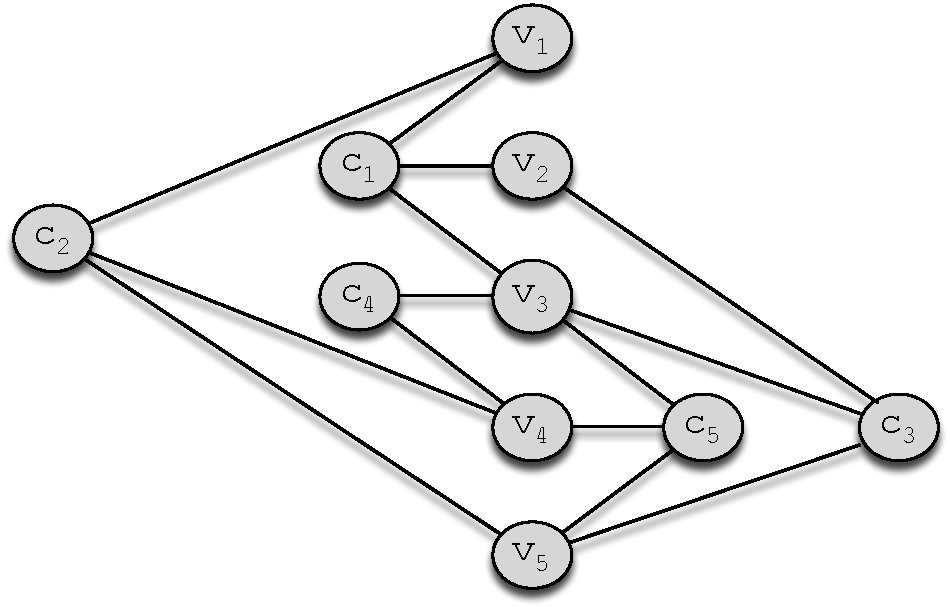
\includegraphics[scale=0.53]{figs/gvarphi.pdf}}
\subfigure[Graph formed using variable gadget from ...]{\label{fig:varphi2}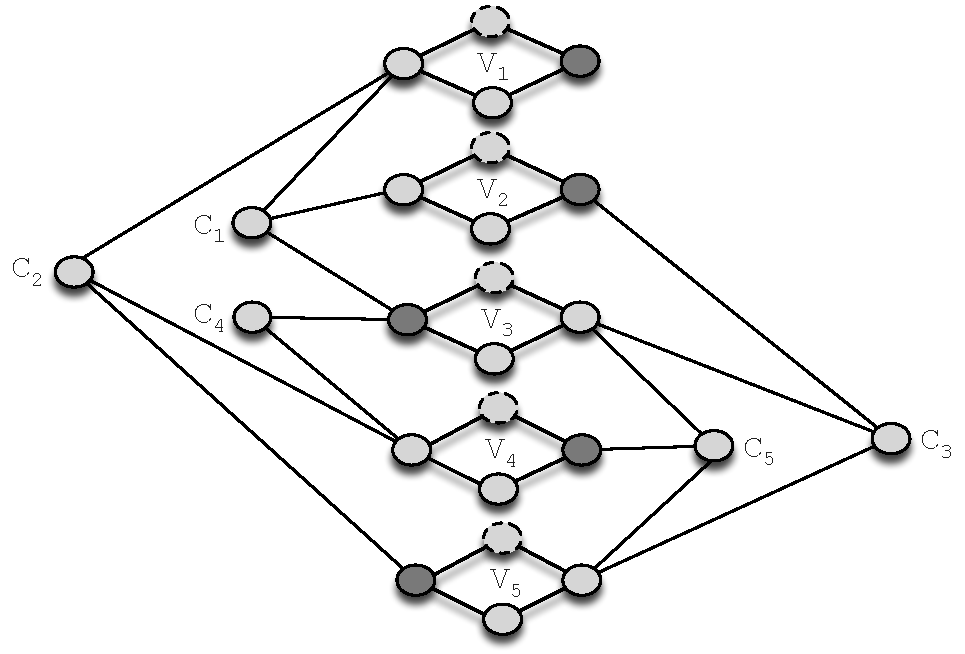
\includegraphics[scale=0.53]{figs/proof1-inject-example.pdf}}

\caption{Example } 
\end{figure}


\begin{figure}[t]
\centering
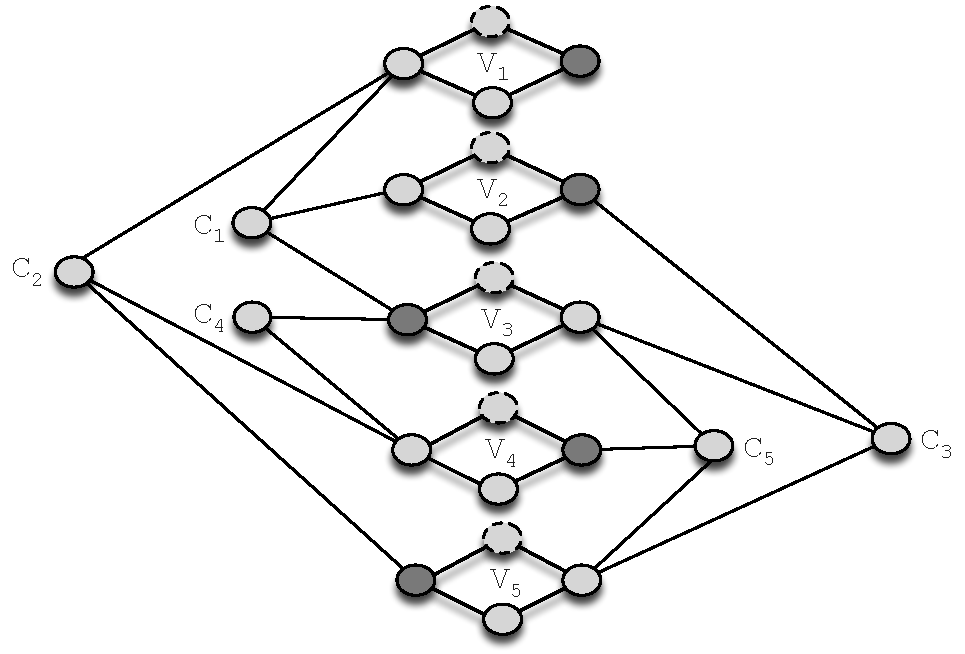
\includegraphics[scale=0.53]{figs/proof1-inject-example.pdf}
%\includegraphics[scale=0.51]{figs/example2.pdf}
\caption{Graph $G=(V,E)=H_1(\varphi)$ formed from $\varphi$ formula in Theorem \ref{thm:npc-full} proof. Nodes with a dashed border are zero-injection nodes.}
\label{fig:proof1-inject-example}
\end{figure}

\begin{figure}[t]
    \fbox{\subfigure[Variable gadget $V_i$ used in Theorem \ref{thm:npc-full} and Theorem \ref{thm:npc-maxinc}.]
	{\label{fig:diamond-gadget}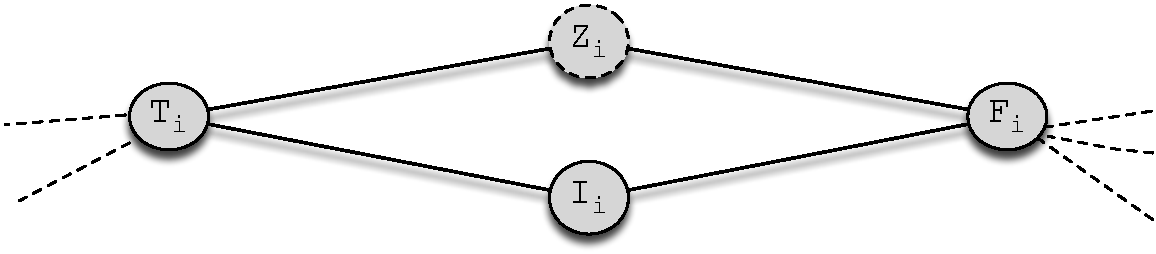
\includegraphics[scale=0.39]{figs/diamond-gadget.pdf}}}
    \fbox{\subfigure[Clause gadget $C_j$ used in Theorem \ref{thm:npc-maxinc}.]
	{\label{fig:line-gadget}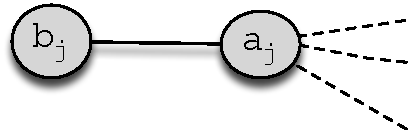
\includegraphics[scale=0.39]{figs/line-gadget.pdf}}}
	\caption{Gadgets used in Theorem \ref{thm:npc-full} and Theorem \ref{thm:npc-maxinc}. $Z_i$ in Figure (a) is the only zero-injection node. The dashed edges in Figure (a) are connections to clause gadgets.  Likewise, the dashed edges in Figure (b) are connections to variable gadgets. }
  \label{fig:pmu-gadgets}
\end{figure}


%\begin{figure}[t]
%\centering
%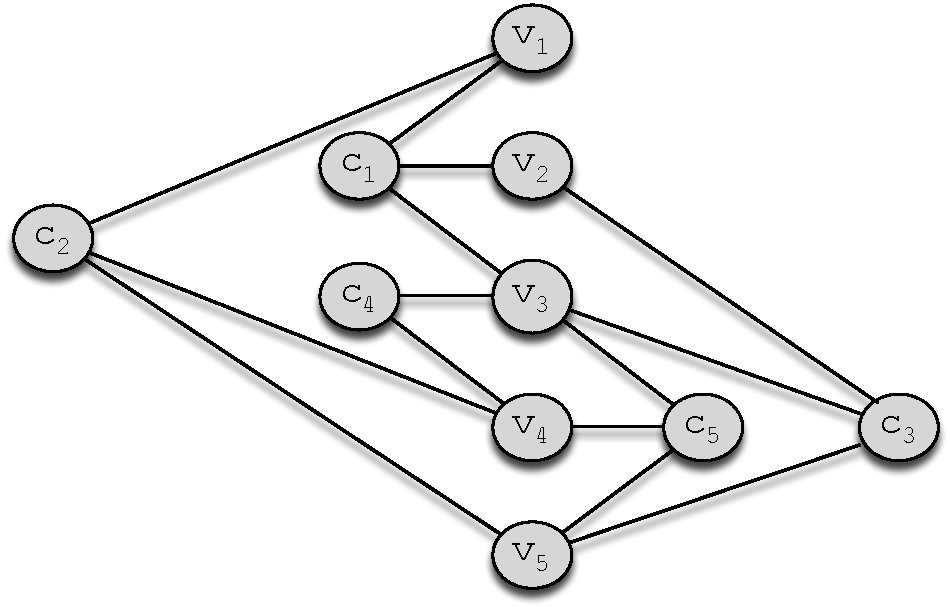
\includegraphics[scale=0.53]{figs/gvarphi.pdf}
%\caption{$G(\varphi)=(V(\varphi),E(\varphi))$ formed from $\varphi$ in Equation (\ref{eqn:varphi}). }
%\label{fig:gvarphi}
%\end{figure}


